\documentclass[12pt,a4paper]{article}

\usepackage{import}
\import{../Template/}{format.tex}

\newcommand{\topic}{Quantum Condensed Matter}
\title{\topic}

\begin{document}

\begin{titlepage}
    \maketitle
\end{titlepage}

\tableofcontents

\newpage

\begin{abstract}
\noindent
Abstract of this course
\end{abstract}

\section{Optical Properties}
We studied the optical properties of materials, including insulators (Using the Lorentz Model) and metals(Using the Drude Model).\\



We also discussed the thermal properties.

Finally, In metals, one of the most important is screening. Note screening is different from dielectric.
\subsection{Insulators}
    The model we used here is Lorentz or dipole oscillator model.\\
    \indent Oscillation of charges around their average position.\\
    \indent Model atoms as nucleus and electron cloud and an applied E-field will lead to the displacement of the electron cloud.\\
    \subsubsection{Lorentz Model}
        Electrons now behave as a damped harmonic oscillator.\\
        \begin{equation}
            m \ddot{u} + m\gamma\dot{u} + m\omega_T^2 u = qE
        \end{equation}
        Natural frequency $\omega_T$ is determined by force constant and mass.
        N.B. $\gamma$ is the damping rate.\\
        The flow of work: for a certain frequency $\omega_T$, we can obtain
        \begin{itemize}
            \item {dipole moment per atom, $p_\omega$}
            \item {Polarisation (dipole moment per unit volume), $P_\omega$}
            \item {Susceptibility, $\chi_\omega$}
            $$
            \chi_\omega=\frac{N}{V} \frac{q^2}{m \epsilon_0\left(\omega_{\mathrm{T}}^2-\omega^2-i \omega \gamma\right)}
            $$
            \item {Permittivity,$\epsilon_\omega$}
            $$
            \epsilon_\omega=1+\chi_\omega
            $$
            \item {Reflectivity between media of different permittivity, power reflection coefficient .etc.}
        \end{itemize}
        At low frequencies, we study the permittivity of the material
        \begin{align}
            \epsilon (\omega\approx 0) = 1+ n_v \frac{q^2}{m\epsilon_0\omega_T^2}
        \end{align}
        This explains the different static permittivity of different materials.\\
        
        \begin{example}
            {Atomic absorption}{?? Something about line width}
        \end{example}
    \subsubsection{Link to quantum mechanics
    }
        

\subsection{Metals}
    Inner electrons closely bounded, contribute to permittivity according to Lorentz oscillator metals.
    Outer electrons have cut loss from ions, now free to roam around the entire metal.
    Natural frequency $\omega_T \approx 0$.
    
\subsection{Drude Model}
    We used Drude Model to study the connectivity of metals (while the Lorentz model to study insulators)
    Drude model is that the electrons are free to move around the metal, and the current is proportional to the electric field. Natural frequency is therefore 0. Also, there is one extra $\epsilon_\infty$ term in the permittivity.
    $$
    \epsilon_\omega=\epsilon_{\infty}-\frac{N}{V} \frac{q^2}{m \epsilon_0\left(\omega^2+i \omega \gamma\right)}=\epsilon_{\infty}-\frac{\omega_{\mathrm{p}}^2}{\omega^2+i \omega \gamma}
    $$
    This is not the correct model (See the real one with drift velocity)
    \subsubsection{Frequency-dependent Connectivity}
        \begin{itemize}
            \item Both current density $\vb{j}= nq\vb{\dot{u}}$, and polarisation $\va{P}=nq\va{u}$.
            \item For conduction electrons $\dot{\vb{P}}_c = \vb{j}$.
            \item The polarization is comprised of core electrons and conduction:
            \item ** Solve PDE $\dot{\vb{P}} = \vb{j} + \epsilon_0 \chi_\infty \dot{\vb{E}}$ and solution with $\vb{E} = \vb{E}_0 e^{-i\omega t}$ **
            \item From this differential equation we have $\vb{j}_\omega = -i\omega \epsilon_0 \vb{E}_\omega (\chi_\omega-\chi_\infty)$
            \item Imaginary part of the permittivity is linked to the real part of frequency-dependent conductivity.
        \end{itemize}

    \subsubsection{ Results from Drude Model}
    Plasma frequency
    $$
    \omega_{\mathrm{p}}^2=\frac{n e^2}{\epsilon_0 m}
    $$
    Frequency dependence of the relative permittivity and electrical conductivity (taking into account the polarisability of the atomic cores, $\chi_{\infty}=\epsilon_{\infty}-1$ causes slight modifications):

    Note that high permittivity means high reflection. Low permittivity means absorption (Highly imaginary $\epsilon$) or transmission (Low $\epsilon$)

    $$
    \begin{gathered}
    \epsilon(\omega)=1-\frac{\omega_{\mathrm{p}}^2}{\omega^2+i \omega \gamma} \stackrel{\epsilon_{\infty} \neq 1}{\longrightarrow} \epsilon_{\infty}-\frac{\omega_{\mathrm{p}}^2}{\omega^2+i \omega \gamma} \\
    \sigma(\omega)=-i \omega \epsilon_0(\epsilon(\omega)-1) \stackrel{\epsilon_{\infty} \neq 1}{\longrightarrow}-i \omega \epsilon_0\left(\epsilon(\omega)-\epsilon_{\infty}\right)
    \end{gathered}
    $$
    Useful expressions for electrical conductivity and Hall coefficient:
    $$
    \begin{gathered}
    \sigma(\omega)=\frac{n e^2 \tau}{m(1-i \omega \tau)} \stackrel{\omega \rightarrow 0}{\longrightarrow} \frac{n e^2 \tau}{m}=n e \mu \\
    R_{\mathrm{H}}= \frac{E_y}{j_x B}=\frac{1}{n q}
    \end{gathered}
    $$
    ( $q$ is carrier charge, $n$ is carrier density, $\tau$ is relaxation time $=1 / \gamma$ )
    \subsubsection{Relaxtion-time approximation}
        We denote relaxation time as $\tau$, and the probability of collision during $\delta t$ is $\delta t/\tau$.
        Now consider the change in \textbf{momentum} change after $\delta t$, by considering electrons collided and not collided during that $\delta t$:\\
        The current $J$ due to electrons of number density $n$, mass $m$ of average (drift velocity) $\vb{v}$ and momentum $\vb{p}$ is given as:
        \begin{equation}
            \vb{j}=-ne\vb{v}=-\frac{ne}{m}\vb{p}
        \end{equation}
        Note that $\vb{J}$ is proportional to $\vb{v}$ and $\vb{p}$.\\
        The evolution of $\vb{p}$ in time $\delta t$ under the action of external force $\vb{f}$, e.g. $\vb{f}=q(\vb{E}+\vb{v}\crossproduct\vb{B})$

        \indent \textbf{Collided electrons} has a fraction $\delta t/\tau$ and momentum is acquired is $\approx \vb{f(t)}\delta t$, as a result, the contribution to the average momentum is of order $(\delta t)^2$:\textbf{negligible}\\
        \indent \textbf{Non-collided electrons}: 
        \begin{equation}
            \vb{p}(t+\delta t) = (1- \delta t/\tau)(\vb{p}(t)+\vb{f}(t)\delta t+ O(\delta t)^2)
        \end{equation}
    \subsubsection{Validity of Drude Model}
    \subsubsection{Summary of key results in Drude Theory}
    \subsection{Sommerfeld Model}
        Both Lorentz and Drude's theories fail dramatically to describe thermodynamic properties. 
        Now we apply the equipartition theorem to the dipole model, expecting a contribution of $k_B$ to the heat capacity of each oscillator, and $3/2k_B$ per atom.
        Also, we consider quantum static effects.
        \subsubsection{Density of states}
            \begin{enumerate}
                \item Fermi sphere
                \item Note spin degeneracy 
                \item $g(E)\equiv$ number of states per unit energy per unit volume.
                \item Number density of electrons $n=\int_0^\infty g(E)f(E)dE$
                \item Internal energy density is $U=\int_0^\infty g(E)E f(E)dE$
                \item $C_v=\frac{dU}{dT}=\int_0^\infty g(E)E\frac{df}{dT}dE$
                \item Note that $C_v$ due to electrons is usually much smaller than lattice-specific heat capacity.
                \item {This is seen in the liquid helium mixture of ${}^{3}He$ and ${}^{4}H$
                \begin{example}
                    {Specific heat of mixture of ${}^{3}He$ and ${}^{4}He$}
                    {We see that at low temp limit, $C_v$ is linear to $T$}
                \end{example}
                }
            \end{enumerate}
        \subsubsection{Screening and the Tomas-Fermi approximation}
            \begin{enumerate}
                \item Screening: placing positive charges in metal will result in electrons moving around to screen its potential resulting in zero electric fields. Compare to dielectric material with electrons are not free to move and have potential reduced by $\epsilon$
                \item A balance is reached between minimizing potential and kinetic energy, screening over a short but finite range.
                \item In order to study the effect of introducing external potential. We study the response of a free electron in a perturbing potential. Free electron in \textbf{METAL}, without external potential, gives potential in the metal to be:
                \begin{equation}
                    \laplacian {V_0}(r) = - \frac{\rho_0(r)}{\epsilon}
                \end{equation}
                indicating that potential is linked to charge distribution. In plasma or Jellium model. $\rho_0 =0$
                \item In the presence of perturbing potential $V_{ext}$, change density will redistribute and we have a perturbing potential in the metal, its correction is :
                \begin{equation}
                    \laplacian \delta{V_0}(r) = - \frac{\delta \rho_0(r)}{\epsilon}
                \end{equation}d
                \paragraph*{Slowly varying potential} 
                The approximation is: Slowly varying potential, and only shifts the free electron.
                \paragraph*{Constant chemical potential}
                keeping the electrons states filled up to a constant energy $\mu$ requires we adjust local Fermi energy $E_F(\vb{r})$:
                \begin{equation}
                    \mu = E_F(\vb{r}) - e V_{tot}(\vb{r})
                \end{equation}
                \paragraph*{Local density approximation}
                    Small shift in the Fermi energy $\delta E_F(\vb{r})$ will give rise to a change in number density, $n$:
                    Recall the then relationship:
                    \begin{equation}
                        \int^{E_F} g_v(E) dE = n
                    \end{equation}
                    we obtain:
                    \begin{equation}
                        \delta n = e g_V(E_F)(\delta V + V_{ext})
                    \end{equation}
                \paragraph*{Lineariesd Thomas Fermi}
                    now we know the small change in $\rho$, as $\rho = e n$
                    We obtain:
                    \begin{equation}
                        \laplacian{\delta V(\vb{r})} = \frac{e^2 g_V(E_F)}{\epsilon_0}(\delta V + V_{ext})
                    \end{equation}
                \paragraph {Density Response}
                    Solve the Equation above, by Fourier Transformation, we obtain:
                    \begin{equation}
                        \delta V(\vb{q}) = -\frac{q^2_{TF}}{q^2+q^2_{TF}}V_{ext}(\vb{q})
                    \end{equation}
                    Here $q_{TF}$ is the \it{Thomas-Fermi Wave vector}
                    The number density, as now we know $\delta V$, 
                \paragraph*{Dielectric permitivity}
                    the dieelctric permitivity $\epsilon_{TF}(q)$
                    \begin{equation}
                        \epsilon_{TF}(q)= 1+ \frac{q_{TF}^2}{q^2}
                    \end{equation}
                \paragraph*{Screening}
                    At small q, long distance, $\epsilon_{TF}$
            \end{enumerate}

\section{Electrons and phonons in periodic solids}
    In this section, we discuss the type of bonds: "Van der Waal", ionic, covalent. Crystal structure
    This is like a section that dedicated to material science
    \subsubsection{Binding of crystals}
        \paragraph*{Inert gas}
        \begin{enumerate}
            \item Filled electron shells and large ionization energies.
            \item Interaction between neutral atoms is weak, and leading attractive force is van der Waals interaction, which gives potential proportional to $1/R^6$.
            \item Lennard-Jones potential:
            \begin{equation}
                U(R) = 4\epsilon[(\dfrac{\sigma}{r})^{12}-(\dfrac{\sigma}{r})^{6}] = \epsilon[(\dfrac{R_{min}}{r})^{12}-2(\dfrac{R_{min}}{r})^{6}]
            \end{equation}
        \end{enumerate}
        \paragraph*{Ionic Crystals}
            \begin{enumerate}
                \item Electrostatic energy for a regular lattice:
                \begin{equation}
                    U_{electrostatic} = -\frac{1}{2}\frac{\alpha_M q^2}{4\pi \epsilon_0 R}
                \end{equation}
                where $\alpha_M$ is a dimensionless constant that depends only on the crystal structure
            \end{enumerate}
    \subsection{Complex materials}
    \subsection{Description of periodic materials}
        \subsubsection{Index system for lattice}
        \subsubsection{Reciprocal Lattice and Diffraction}
        \subsubsection{Diffraction Condition}
        The spacing 
        \begin{equation}
            2 d \sin \theta=n \lambda
        \end{equation}
\subsection{Lattice dynamics and phonons}
\paragraph{1D monatomic chain}
\paragraph{1D diatomic chain}
\paragraph{1D different spring constant}
\paragraph{1D different mass}
\paragraph{3D crystal}
In 3D crystal, there are always 3 acoustic modes and 3(m-1) optical modes where m is the number of atoms per unit cell.
\subsection{Density of states}
\subsection{Heat Capacity} 
    When studying heat capacities, we discuss the optical branch (Einstein Model)and acoustic model (Debye model)
    \subsubsection{Debye Model}
    2.8 Lattice-specific heat
    Phonons obey Bose-Einstein statistics, but their number is not conserved and so the chemical potential is zero, leading to the Planck distribution
    $$
    n(\omega)=\frac{1}{\exp \left(\hbar \omega / k_{\mathrm{B}} T\right)-1}
    $$
    The internal energy is
    $$
    U=\int d \omega D(\omega) n(\omega) \hbar \omega
    $$
    For the Einstein model
    $$
    U_E=\frac{N \hbar \omega_o}{\mathrm{e}^{\hbar \omega_o / k_{\mathrm{B}} T}-1}
    $$
    and the heat capacity is
    $$
    C_V=\left(\frac{\partial U}{\partial T}\right)_V=N k_{\mathrm{B}}\left(\frac{\hbar \omega_o}{k_{\mathrm{B}} T}\right)^2 \frac{\mathrm{e}^{\hbar \omega_o / k_{\mathrm{B}} T}}{\left(\mathrm{e}^{\hbar \omega_o / k_{\mathrm{B}} T}-1\right)^2}
    $$
    At low temperatures, this grows as exp $-\hbar \omega_o / k_{\mathrm{B}} T$ and is very small, but it saturates at a value of $N k_{\mathrm{B}}$ (the Dulong and Petit law) above the characteristic temperature $\theta_E=\hbar \omega_o / k_{\mathrm{B}} \cdot{ }^6$

    At low temperatures, the contribution of optical modes is small, and the Debye spectrum is appropriate. This gives
    $$
    U_{\mathrm{D}}=\int_0^{\omega_{\mathrm{D}}} d \omega \frac{V \omega^2}{2 \pi^2 v^3} \frac{\hbar \omega}{\mathrm{e}^{\hbar \omega / k_{\mathrm{B}} T}-1}
    $$
    Defining the Debye temperature $\theta_{\mathrm{D}}=\hbar \omega_{\mathrm{D}} / k_{\mathrm{B}} T$ and using $\omega_{\mathrm{D}}^3=6 \pi^2 v^3 N / V$ from above, we obtain $\theta_{\mathrm{D}}=\left(6 \pi^2 N / V\right)^{1 / 3} \hbar b / k_{\mathrm{B}}$. \\
    By writing $x=\hbar \omega / k_{\mathrm{B}} T$ and including a factor of 3 for different modes, we obtain for the internal energy
    $$
    U_{\mathrm{D}}=\frac{3 V \hbar}{2 \pi^2 v^3} \int_0^{\omega_{\mathrm{D}}} d \omega \frac{\omega^3}{\mathrm{e}^{\hbar \omega / k_{\mathrm{B}} T}-1}=9 N k_{\mathrm{B}} T \frac{T}{\theta_{\mathrm{D}}} \int_0^{\theta_{\mathrm{D}} / T} d x \frac{x^3}{\mathrm{e}^x-1}
    $$
    and by differentiating the middle expression with respect to temperature, the heat capacity (see Fig. 2.29) is
    $$
    C_V=9 N k_{\mathrm{B}}\left(\frac{T}{\theta_{\mathrm{D}}}\right)^3 \int_0^{\theta_{\mathrm{D}} / T} d x \frac{x^4 \mathrm{e}^x}{\left(\mathrm{e}^x-1\right)^2}
    $$
    where the Debye temperature is $\theta_{\mathrm{D}}=\hbar \omega / k_{\mathrm{B}}$. We have multiplied by 3 to account for the three acoustic branches.
    \subsubsection{Heat capacity due to lattice vibration and electrons}
    Two major contributions to heat capacity: electrons and lattice vibrations. Electron heat capacity is linear to $T$ ??? while lattice vibration heat capacity is $\propto T^3$
    \subsubsection{Compare Einstein and Debye models}
    Why we are comparing these two models???
\subsection{Thermal Conductivity of insulators}
    \begin{enumerate}
        \item The thermal conductivity, $\kappa$ is defined by $\boldsymbol{J}_q=-\kappa \nabla T$, where $\boldsymbol{J}_q$ is the flux of heat (energy per unit area per unit time).
        \item Kinetic theory gives $\kappa=\frac{1}{3} C_{\mathrm{V}} \ell v=\frac{1}{3} C_{\mathrm{V}} v^2 \tau$, where $C_{\mathrm{V}}$ is the phonon specific heat per unit volume, $v$ is the phonon velocity, $\ell=v \tau$ is the mean free path and $\tau$ is the scattering time. 
        \item Debye theory predicts that $C_{\mathrm{V}} \propto T^3$ \textbf{at low $T$} and that it is constant at high $T$(While in reality, at high temperature, thermal conductivity is dominated by scattering). 
        \item $v$, the velocity of sound, is almost constant, but $\tau$ depends on several scattering mechanisms. 
        \item Scattering Mechanisms include normal, Umklapp, points defects sample boundaries and crystal dislocations.
        \item At high temperaturem $\kappa$ falls rapidly due to rapid fall in $\tau$, the scattering time. 
    \end{enumerate}
\section{Electrons in periodic potential}
    By solving Hamiltonian's equation, we conclude Bloch's theorem: Eigenstates of the 1D Hamiltonian can be chosen to be a plane wave multiplied by a function with the periodicity of the Bravais lattice.\\
    We consider first a formal treatment in terms of a complete set of basis functions, namely the set of all plane-wave states which satisfy the periodic boundary conditions. The results from this treatment can be used to obtain Bloch's theorem, which is one of the cornerstones of electronic structure in solids. Next, we will approach Bloch's theorem from a more abstract but also more elegant direction, which uses the translational symmetry of the lattice directly.

\subsection{Shrodinger equation ina periodic table}
\subsection{Bloch theorem from discrete translational symmetry}
Another way to think about Bloch theorem, consider what happens to eigenstate of Hamiltonian.\\ 

The underlying reason is that if an operator is unchanged under a change of coordinate system, then applying a symmetry operation on the eigenstate of such an operator produces another eigenstate of the operator, with the same eigenvalue as the original one.\\

For two commuting operators H and T, we can always choose simultaneous eigenstates of both H and T 

Two forms of Bloch theorem:
$$
\psi_{\boldsymbol{q}}(\boldsymbol{r})=\mathrm{e}^{\mathrm{i} \boldsymbol{q} \cdot \boldsymbol{r}} \sum_{\boldsymbol{G}} c_{\boldsymbol{q}-\boldsymbol{G}} \mathrm{e}^{-\mathrm{i} \boldsymbol{G} \cdot \boldsymbol{r}}=\mathrm{e}^{\mathrm{i} \boldsymbol{q} \cdot \boldsymbol{r}} u_{j, \boldsymbol{q}}(\boldsymbol{r})
$$            

$$
\psi_{\boldsymbol{k}}^{(n)}(\boldsymbol{r}+\boldsymbol{R})=\mathrm{e}^{\mathrm{i} \boldsymbol{k} \cdot \boldsymbol{R}} \psi_{\boldsymbol{k}}^{(n)}(\boldsymbol{r})
$$
\subsection{Tight banding}
A tight band is also called a linear combination of atomic orbitals.\\
\subsubsection{Two Bands}
In this section, we consider tight binding - two bands. For example, s-band or d-band.
We approach this problem by forming two Bloch states, one from each set of atomic orbital
      
\subsection{Band Structure and Brillioun Zone}
\paragraph*{Brillouin Zone}
We found that the energy eigenstates formed discrete bands $E_n(\boldsymbol{k})$, which are continuous functions of the momentum $\boldsymbol{k}$ and are additionally labeled by a band index $n$. The bandstructure is periodic in the reciprocal lattice $E_n(\boldsymbol{k}+\boldsymbol{G})=E_n(\boldsymbol{k})$ for any reciprocal-lattice vector $\boldsymbol{G}$. It is sometimes useful to plot the bands in repeated zones, but remember that these states are just being relabelled and are not physically different.
\paragraph*{Crystal Momentum}
The quantity $\hbar \boldsymbol{k}$ is the crystal momentum, and it enters conservation laws for scattering processes. For example, if an electron absorbs the momentum of a phonon of wavevector $\boldsymbol{q}$, the final state will have a Bloch wavevector $\boldsymbol{k}^{\prime}=\boldsymbol{k}+\boldsymbol{q}+\boldsymbol{G}$, where $\boldsymbol{G}$ is whatever reciprocal lattice vector necessary to keep $\boldsymbol{k}^{\prime}$ inside the Brillouin zone. Physical momentum can always be transferred to the lattice in arbitrary units of $\hbar \boldsymbol{G}$. Notice that depending on the energy conservation, processes can thus lead to transitions between bands.
\paragraph*{title}

\subsubsection{Example of Band Structures}    
\subsection{Semiclassical Model of electron dynamcis}
\section{Experimental Probe of the band structure}
The system can be excited in different ways: absorption of photon/ or photon + phonon.
Photons will appear vertically and phonons are horizontal on plots of energy against $k$.

The minimum gap in a semi-conductor is the energy difference between the highest occupied state and the lowest unoccupied state, and this is the threshold for optical absorption.

Maximum valence band states and the minimum band state can occur at the same or different momentum.

Examples of the indirect band gap is Si and Ge. A \textbf{Phonon-mediated} transition is required and
\subsection{Photon Absorption}
\subsubsection{Transitioon rates}
Ferim's Golden Rule:
$W_{\mathrm{i} \rightarrow \mathrm{f}}=\frac{2 \pi}{\hbar}|M|^2 g(\hbar \omega)$
which depends on the dipole matrix element $M$ and the density of states $g$.

The matrix element is calculated using the initial and final states and the perturbation due to interaction of electric field of the photon and the electric dipole moment $P$
\note{Why there is a dipole moment}

We calculate the matrix element by integrating over the whole crystal:
$$
M=\frac{e}{V} \int u_{\mathrm{f}}^*(\boldsymbol{r}) \mathrm{e}_0^{\mathrm{i} \boldsymbol{k}_{\mathrm{f}} \cdot \boldsymbol{r}}\left(\boldsymbol{E}_0 \cdot \boldsymbol{r} \mathrm{e}^{\mathrm{i} \boldsymbol{k} \cdot \boldsymbol{r}}\right) u_{\mathrm{i}} *(\boldsymbol{r}) \mathrm{e}^{\mathrm{i} \boldsymbol{k}_{\mathrm{i}} \cdot \boldsymbol{r}} \mathrm{d}^3 \boldsymbol{r} .
$$
This is expression is symplified as conservation of momentum so the phase factor must be zero.

Photon absorption is vertical on the E-K diagram as the eavevector of photon is much lower than the wavevector if electron states.
\subsubsection{GaAs band structure}
As
\subsubsection{Transition rate- joint density of states}
Back to the Transition rate, the factor g that appears in Fermi golden rule is the joint density of states, due to the facto that bot initial and final states lie in continueous bands. 

$$
\begin{aligned} 
    & \hbar \omega<E_{\mathrm{g}}=g(\hbar \omega)=0 \\ & \hbar \omega>E_{\mathrm{g}}=g(\hbar \omega)=\left(\frac{1}{2 \pi^2}\right)\left(\frac{2 \mu}{\hbar^2}\right)^{3 / 2} \sqrt{\hbar \omega-E_{\mathrm{g}}}
\end{aligned}
$$
\subsubsection{Transition rate in direct semiconductors}
$\alpha \propto \sqrt{\hbar \omega-E_g}$ is the theroetical rate of absorption while in reality it is hardly obeyed.
\begin{enumerate}
    \item Columb attraction beterrn electrons and holes, which inhances absorption and leading to formation of a bound pair - exciton.
    \item Impurities and defects with energyies within the bandgap.
\end{enumerate}
\paragraph{Excitons}
An exciton is a bound electron-hole pair analogous to the hydrogen atom. In an exciton, electron and heavy-hole masses are combined in a reduced effective mass
$$
\frac{1}{\mu^*}=\frac{1}{m_{\mathrm{e}}^*}+\frac{1}{m_{\mathrm{hh}}^*}
$$
GaAs has permittivity $\varepsilon=12.8$. We can use a modified equation for the energy levels of a hydrogen atom to calculate energy levels of excitons:
$$
E_n=-\frac{\mu^*}{m_{\mathrm{e}} \varepsilon^2} \cdot \frac{13.6 \mathrm{eV}}{n^2}=-\frac{R_x}{n^2}
$$
The energy $\varepsilon_n$ of an exciton is equal to the energy required to create an electron-hole pair, minus the binding energy or
$$
\varepsilon_n=E_{\mathrm{g}}-\frac{R_x}{n^2}
$$
\subsubsection{Transition rate in Indirect semiconductors}
Semiconductors like Si and Ge have their conduction abnd minimun away from teh BZ centere and the valence band maximum. A transisition between band edges need a big change in electron wavevector.

Transition from electron ($\left(\varepsilon_i, k_1\right)$) to 

The absoprtion rate is a second order process, meaning that the rate fr indirect semiconductors is much smaller.
absorption coefficient $\alpha(\hbar \omega) \propto\left(\hbar \omega-E_{\mathrm{g}} \mp \hbar \Omega\right)^2$ has a frequency (of Phonon) dependency, which is not seen in direct bandgap semiconductors.

\subsection{Photoemission}
Most direct way too measure electron spectral function.
\begin{enumerate}
    \item Photon incident on a solid, cause transitions from occupied states to plane-wave-like states.
    \item excited electrons leave the crystal and is collected by the detector to analyze its energy and momentum. 
    \item Determine the band structure directly.
\end{enumerate}
Note that momentum parallel to the surface is conserved.
\subsection{STM}
\subsection{Cyclotron Resonance}
\section{Scattering in metals}
We consider the scattering in metal with isotropic bands characterized by an effective mass and a spherical Fermi surface.
\begin{enumerate}
    \item Electrical conductivity
    \item thermal conductivity (dependent on T)
    \item electronic specific heat capacity
\end{enumerate}
\theorem{Wiedemann-Franz law}{The ratio of the thermal conductivity and the electrical conductivity is proportional to the temperature}
We further discuss this issue wit electrical and thermal transport.
\begin{enumerate}
    \item electrical transport
    \item thermal transport: Long arrow
    \item Long arrow means changed direction of electrons which both affect thermal and electrical transport
    \item Short arrow only appears for short arrow in the low temperature
\end{enumerate}
\subsection{Matthiessen's rule}
The scattering process with the shortest scattering time will dominate.
An application for the Matthiessen's rule is the calculation of electron mobility in 2D electron gases for different scattering processes
\subsection{Emission and absorption of phonons}
Phonons, we picture them as propagating local distortion of the crystal, which may scatter an electron in two different ways: elastic and inelasitc (Conseravation of momentum)
So far we assumed he positions of ions are not affected, while it is not true in general. Electronsin with distort the lattice -- as if they emiited a phonon.
Phonons have blackbody distribution with energy of order $k_B T$
\subsubsection{Electron-phonon scattering at room temperature}
A phonon can scatter electron to the other side of Fermi surface (Recall the long arrow in the electrical and thermal transport)
\subsubsection{Electron-phonon scattering at low temperature}
Energy of phonon is to little to chaneg direction. In this case electrical scattering rate is much less than teh thermal scattering rate.
Hence we have $\tau_\sigma^{-1} \propto T^5$ and $\tau_\kappa^{-1} \propto T^3$ and so $\tau_\sigma^{-1} \ll \tau_\kappa^{-1}$ at low $T$.
\paragraph*{Umklapp}
Scattering into the neighboring Brillouin Zone.

\begin{tabular}{|c|c|c|c|}
    \hline $\begin{array}{l}\text { Temperature } \\
    \text { (scatterer) }\end{array}$ & $\begin{array}{l}\text { Scattering } \\
    \text { times }\end{array}$ & $\begin{array}{l}-1+2 \\
    \sigma \\
    \sigma\end{array}$ & W-F ratio \\
    \hline $\begin{array}{l}\text { Very low } \\
    \text { (impurities) }\end{array}$ & $\begin{array}{l}\tau_\kappa \approx \tau_\sigma \\
    \sim \text { const }\end{array}$ & $\begin{array}{l}\kappa \propto T \\
    \sigma \sim \text { const }\end{array}$ & $L_0$ \\
    \hline $\begin{array}{l}T \sim \theta_{\mathrm{D}} / 10 \\
    \text { (phonons) }\end{array}$ & $\begin{array}{l}\tau_\kappa \propto T^{-3} \\
    \tau_\sigma \propto T^{-5} \rightarrow e^{-\theta_{\mathbf{F}} / T}\end{array}$ & $\begin{array}{l}\kappa \propto T^{-2}, \\
    \sigma \propto T^{-5} \rightarrow e^{-\theta_{\mathrm{F}} / T}\end{array}$ & $<L_0$ \\
    \hline $\begin{array}{l}T>\sim \theta_{\mathrm{D}} \\
    \text { (phonons) }\end{array}$ & $\begin{array}{l}\tau_\kappa \approx \tau_\sigma \\
    \propto T^{-1}\end{array}$ & $\begin{array}{l}\kappa=\text { const, } \\
    \sigma \propto T^{-1}\end{array}$ & $L_0$ \\
    \hline
\end{tabular}

\subsubsection{Electron-electron scattering}
Relatively Unimportant
Conservation of energy/momentum

\section{Quantum Oscillations}
\subsection{Size of Cyclotron orbits}
The flux threading the real space 
Area enclosed by the k-space orbital:
$$
A_k=\left(\frac{e}{\hbar}\right)^2 B^2 A_r
$$

$$
A_k=\frac{2 \pi e}{\hbar} B\left(n+\frac{1}{2}\right)
$$
\subsection{Density of states}
Period of Oscillation:
$$
\Delta\left(\frac{1}{B}\right)=\frac{1}{B_{n+1}}-\frac{1}{B_n}=\frac{2 \pi e}{\hbar} \frac{1}{A_k}
$$
This links the period of quantum oscillations to the cross-sectional area of Fermi Surface.
\subsection{De-Hass Van-Alphen effect}
\subsection{De-Hass Van-Alphen effect in Sr2RuO4}
\subsection{Tunneling}
I will not study this part 
\subsection{Cyclotron Resonance}

\section{Semiconductor band structure}
Direct gap vs Indirect gap
\begin{enumerate}
    \item Direct gap: $k=0$
    \item Indirect gap: $k\neq 0$, local minimum at the origin of the reciprocal lattice. Global minimun at $k = \eta$
\end{enumerate}
\subsection{Intrinsic carrier concentration}
Semicondoctors are material with small energy gap. So small that the thermal energy is large enough to excite electrons from the valence band to the conduction band.
\begin{enumerate}
    \item Dispersion relationship
    \item Density of states for conduction band and valence band:
    \item Carrier density:
    $$
    n=\int_{E_{\mathrm{c}}}^{\infty} d E g_{\mathrm{e}}(E) f(E)
    $$
    with Fermi function
    $$
    f(E)=\frac{1}{\mathrm{e}^{(E-\mu) /\left(k_{\mathrm{B}} T\right)}+1} \approx \mathrm{e}^{-(E-\mu) /\left(k_{\mathrm{B}} T\right)}
    $$
    \item Concentration of electrons$$
    n \approx 2\left(\frac{m_{\mathrm{e}}^* k_{\mathrm{B}} T}{2 \pi \hbar^2}\right)^{0 / 2} \mathrm{e}^{-\frac{E_{\mathrm{c}}-\mu}{k_{\mathrm{B}} T}}
    $$
    the concentration of holes
    $$
    p \approx 2\left(\frac{m_{\mathrm{h}}^* k_{\mathrm{B}} T}{2 \pi \hbar^2}\right)^{3 / 2} \mathrm{e}^{-\frac{\mu-E_{\mathrm{v}}}{k_{\mathrm{B}} T}}
    $$
    \item define $n_c $and $p_c$:
    $$
    n=n_{\mathrm{c}}(T) \mathrm{e}^{-\frac{E_{\mathrm{c}}-\mu}{k_{\mathrm{B}} T}}
    $$ 
    $$
    p=p_{\mathrm{v}}(T) \mathrm{e}^{-\frac{\mu-E_{\mathrm{v}}}{k_{\mathrm{B}} T}}
    $$
    \item Note that $np$ is constant
    $$
    n p=n_{\mathrm{c}}(T) p_{\mathrm{v}}(T) \mathrm{e}^{-\frac{E_g}{k_{\mathrm{B}} T}}
    $$
    \item Energy gap = Ec -eV
    $$
    E_{\mathrm{g}}=E_{\mathrm{c}}-E_{\mathrm{v}} \simeq 1 e V
    $$
    where $E_g$ is size of the energy gap law of mass action
\end{enumerate}
The only assumption made is that the distance of the Fermi level from the edge of both bands is large in comparison to kBT, this is true in the presence of impurities and dopants.
\subsection{Doped Semicondoctors}
Carriers can also be created in semiconductors by adding impurity atoms in a process called doping
The binding energy of the impurity level:
$$
\Delta_{\mathrm{d}}=\frac{e^4 m_{\mathrm{c}}^*}{2\left(4 \pi \varepsilon \varepsilon_o \hbar\right)^2}=\frac{m_{\mathrm{c}}^* / m_{\mathrm{e}}}{\varepsilon^2} \times 13.6 \mathrm{eV}
$$
which can be very small compared to the band gap, and often comparable or smaller than thermal energies. Such donor impurities readily donate electrons to the conduction band.
\subsection{Hall effect}
Relaxation time approximation:
$$
\frac{\mathrm{d} \boldsymbol{j}}{\mathrm{d} t}=-\frac{\boldsymbol{j}}{\tau}+\frac{n e^2}{m}(\boldsymbol{E}+\boldsymbol{v} \times \boldsymbol{B})
$$
Therefore, in the steady state, for electrons,
$$
\boldsymbol{j}_{\mathrm{e}}=\frac{n e^2 \tau_{\mathrm{e}}}{m_{\mathrm{e}}}\left(\boldsymbol{E}(t)+\boldsymbol{v}_{\mathrm{e}} \times \boldsymbol{B}\right)=n e \mu_{\mathrm{e}}\left(\boldsymbol{E}(t)+\boldsymbol{v}_{\mathrm{e}} \times \boldsymbol{B}\right)
$$
If both electrons and holes are present, we have
$$
\boldsymbol{j}_{\mathrm{e}}=n e \mu_{\mathrm{e}}\left(\boldsymbol{E}+\boldsymbol{v}_{\mathrm{e}} \times \boldsymbol{B}\right)+p e \mu_{\mathrm{h}}\left(\boldsymbol{E}+\boldsymbol{v}_{\mathrm{h}} \times \boldsymbol{B}\right)
$$
If we choose the current to be flowing in the $x$-direction, and $\boldsymbol{B}$ to be in the $z$-direction, then $v_x^{\mathrm{e}}$ and $v_x^{\mathrm{h}}$ have opposite signs and, using $\mu=v / E$, we have
$$
\begin{aligned}
j_x & =e E_x\left(n \mu_{\mathrm{e}}+p \mu_{\mathrm{h}}\right) \\
0 & =e E_y\left(n \mu_{\mathrm{e}}+p \mu_{\mathrm{h}}\right)-e B\left(n \mu_{\mathrm{e}} v_x^{\mathrm{e}}+p \mu_{\mathrm{h}} v_x^{\mathrm{h}}\right) 
\end{aligned}
$$
Eliminating $E_x$ we get
$$
E_y=\frac{j_x B\left(n \mu_{\mathrm{e}}^2-p \mu_{\mathrm{h}}^2\right)}{e\left(n \mu_{\mathrm{e}}+p \mu_{\mathrm{h}}\right)^2}
$$
Now, we can define the Hall coefficient:
$$
R_{\mathrm{H}}=\frac{E_y}{j_x B}=\frac{\left(n \mu_{\mathrm{e}}^2-p \mu_{\mathrm{h}}^2\right)}{e\left(n \mu_{\mathrm{e}}+p \mu_{\mathrm{h}}\right)^2}
$$
\subsection{Semicondoctor devices}
For bulk devices we will use the semiclassical approximation, treating electrons as classical particles governed by the Hamiltonian
$$
H=E_n(\boldsymbol{k})-e \phi(\boldsymbol{r})
$$
with the momentum $\boldsymbol{p}=\hbar \boldsymbol{k}$ and a spatially varying electrostatic potential $\phi(\boldsymbol{r})$. The potential will arise from externally applied fields, from charges induced by doping, and from changes in the material composition.

For an isolated solid in equilibrium, the energy difference between the chemical potential $\mu$ and the vacuum level is the work function $\Phi$. This is the energy required to remove an electron from the Fermi level and place it in a state of zero kinetic energy in free space.

Two different isolated materials with different work functions will then have different chemical potentials. If these two materials are placed in contact, their chemical potentials must equalise, which is accomplished by electron flow to the more electronegative material; this material becomes charged, its potential $\phi$ changes, and an overall balance will be established. But in general, there will be as a result internal inhomogeneous electric fields.

\subsection{Metal}

\subsection{P-N Junction}
A pn junction is formed by inhomogeneous doping: a layer of n-type placed near p-type.
Joining two regions gives a step in chemical potential $\mu$, causing the current to flow.
\begin{figure}[h]
    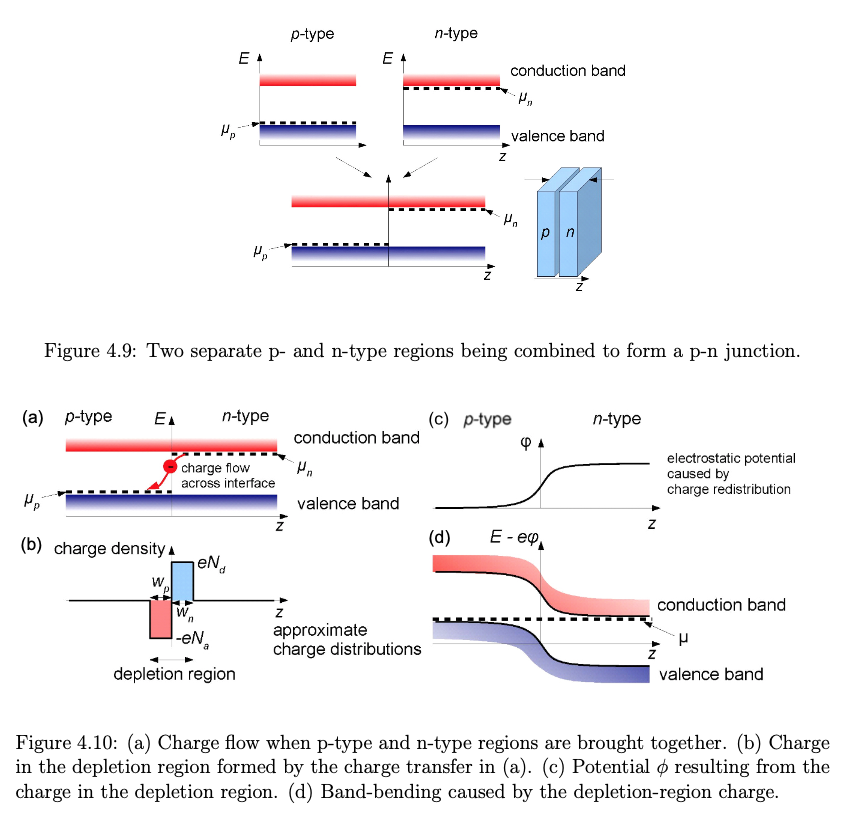
\includegraphics[clip=true,width=\columnwidth]{Images/PN_junction.png}
    \caption{}
\end{figure}
\subsection{Band-bending}
Charge redistribution causes a spatial varying electrostatic potential, energy level shifts from $E$ to $E-e\phi$. The potential satisfies Poisson's equation:
$$
\nabla^2 \phi=\frac{\partial^2 \phi}{\partial z^2}=-\frac{\rho}{\varepsilon \varepsilon_0}
$$
with boundary condition: Far away from the junction in the n-type region, $\mu$ is close to the top of the bandgap and in the p-type region it is close to the bottom of the bandgap.
The junction potential $\phi_{\mathrm{j}}$ (often called $V_{\mathrm{b}}$ ) is defined via $e \phi_{\mathrm{j}}=$ $\mu_{\mathrm{n}}-\mu_{\mathrm{p}}=E_{\mathrm{g}}$. 
From charge neutrality, i.e., the requirement that there is as much negative charge on one side of the depletion region as a positive charge on the other side, we have
$$
N_{\mathrm{A}} w_{\mathrm{p}}=N_{\mathrm{D}} w_{\mathrm{n}}
$$
where $N$ and $w$ are thickness and doping densities.
\subsection{LED, Solar, TFFT, MFFT. etc}

\subsection{Two-dimensional electron gas}
Electrons will fill the state up to Fermi Energy

When applying magnetic field, it splits into Landau levels, and the energy of the Landau levels is given by
$$
E_{n}=\left(n+\frac{1}{2}\right) \hbar \omega_{c}
$$, where $\omega_c$ is the cyclotron frequency.
Each LL has the same degeneracy.
The average density of states per unit area per Landau Level is given by
$$
g = \frac{2n_L}{\hbar \omega_c}
$$, 2 is from spin degeneracy.
This is the same for B= 0:
$$
g(E) = \frac{m}{\pi \hbar^2}
$$
We solve for $n_L$
$$
n_L = \frac{e B}{h}
$$
If there are $\nu$ filled Landau levels at a field $B$, the total density of electrons per unit area is given by
$$
n_{\mathrm{e}}=\frac{\nu e B}{h}
$$
Suppose there are $\nu$ occupied Landau levels at field $B_1$. Then $n_{\mathrm{e}}=\frac{\nu e B_1}{h}$. If the field is increased from $B_1$ to $B_2$ and the highest Landau level is depopulated, the electrons are redistributed among $\nu-1$ levels. Hence $n_{\mathrm{e}}=\frac{\nu e B_1}{h}=\frac{(\nu-1) e B_2}{h}$. On eliminating $\nu$
$$
n_{\mathrm{e}}=\frac{e}{h}\left(\frac{1}{B_1}-\frac{1}{B_2}\right)^{-1} \text {. }
$$
This means that the depopulation of the Landau levels is periodic in $1 / B$, as in 3D.
\subsection{The Quantum Hall effect}
\section{Electronic Instabilities}
\subsection{Curie law of susceptibility}
$$
\chi=\frac{n \mu_0 \mu^2}{3 k_{\mathrm{B}} T}
$$

We consider a local moment $\boldsymbol{m}$ of fixed magnitude $\mu=|\boldsymbol{m}|$, in a small applied magnetic field $\boldsymbol{H} \rightarrow \mathbf{0}$. The dipole energy of this moment is given by $E=-\mu_0 \boldsymbol{m} \cdot \boldsymbol{H}$. There are no discrete states, so this corresponds to $J=\infty$, but the system still relies on QM, as one can only have fixed moments in QM.

Consider magnetic moments $\mu$ at an angle $\theta$ to the applied field. The energy $E=-\mu \cdot \boldsymbol{B}=$ $-\mu B \cos \theta$, and the Boltzmann factor is $\exp \frac{\mu B \cos \theta}{k_{\mathrm{B}} T}$. The probability of the angle lying between $\theta$ and $\theta+\mathrm{d} \theta$ is proportional to
$$
\exp \frac{\mu B \cos \theta}{k_{\mathrm{B}} T} \times \frac{1}{2} \sin \theta \mathrm{d} \theta \quad \text { (including the fraction of solid angle). }
$$

The average moment parallel to $\boldsymbol{B}$ is given by
$$
\left\langle\mu_z\right\rangle=\frac{\int_0^\pi \mu \cos \theta \exp \left(\mu B \cos \theta / k_{\mathrm{B}} T\right) \frac{1}{2} \sin \theta \mathrm{d} \theta}{\int_0^\pi \exp \left(\mu B \cos \theta / k_{\mathrm{B}} T\right) \frac{1}{2} \sin \theta \mathrm{d} \theta}=\frac{\int_{-1}^1 x \exp (y x) \mathrm{d} x}{\int_{-1}^1 \exp (y x) \mathrm{d} x}
$$

This gives the Langevin function (see Fig. 5.9)
$$
\frac{\left\langle\mu_z\right\rangle}{\mu}=\operatorname{coth} y-\frac{1}{y}=\frac{M}{M_{\mathrm{s}}} .
$$
The saturation magnetization $M_{\mathrm{s}}=n \mu$ occurs when all $n$ moments per unit volume are aligned, which will happen when $\mu B / k_{\mathrm{B}} T \gg 1$.
As $y=\frac{\mu B}{k_{\mathrm{B}} T} \rightarrow 0$
$$
\operatorname{coth} y \approx \frac{1}{y}+\frac{y}{3} \quad \Longrightarrow \quad \operatorname{coth} y-\frac{1}{y} \approx \frac{y}{3}
$$
Hence
$$
\frac{M}{M_{\mathrm{s}}}=\frac{\left\langle\mu_z\right\rangle}{\mu} \approx \frac{y}{3}=\frac{\mu B}{3 k_{\mathrm{B}} T}
$$
Since, in small magnetic fields,
$$
\chi=M / H \approx\left(\mu_0 M\right) / B \quad \text { and } \quad M_{\mathrm{s}}=n \mu
$$
\section{Fermi-Liquid Theory}
\subsection{Band Magnetism in metals}
Let us start with Pauli paramagnetism-the response of a metal to an applied magnetic field. We consider a Fermi gas with energy dispersion $\epsilon_{\boldsymbol{k}}$ in a magnetic field $H$. In a magnetic field, the spin-up and spin-down bands will be Zeeman-split (see Fig. 5.17):
$$
\begin{aligned}
& \epsilon_{\boldsymbol{k} \uparrow}=\epsilon_{\boldsymbol{k}}-\mu_{\mathrm{B}} B_{\mathrm{a}} \\
& \epsilon_{\boldsymbol{k} \downarrow}=\epsilon_{\boldsymbol{k}}+\mu_{\mathrm{B}} B_{\mathrm{a}}
\end{aligned}
$$
Since the chemical potential must be the same for both spins, there must be a transfer of carriers from the minority spin band to the majority spin band:
$$
n_{\uparrow}-n_{\downarrow}=2 \mu_{\mathrm{B}} B_{\mathrm{a}} \frac{1}{2} g_{\mathrm{v}}\left(E_{\mathrm{F}}\right)=\mu_{\mathrm{B}} B_{\mathrm{a}} g_{\mathrm{v}}\left(E_{\mathrm{F}}\right)
$$
where $g_{\mathrm{v}}\left(E_{\mathrm{F}}\right)$ is the density of states at the Fermi level per unit volume..$^3$ We could relate $g_{\mathrm{v}}$ to the density of states per atom as $g_{\mathrm{v}}=\frac{N}{V} g$. The magnetisation is $M=\mu_{\mathrm{B}}\left(n_{\uparrow}-n_{\downarrow}\right)$, and $B_{\mathrm{a}}=\mu_0 H$, which gives the static spin susceptibility
$$
\frac{M}{H}=\chi_\sigma=\mu_0 \mu_{\mathrm{B}}^2 g\left(E_{\mathrm{F}}\right)
$$

Now let us include in a very simple fashion the effect of interactions. The Stoner-Hubbard model, which provides arguably the simplest way forward, includes an energy penalty $U$ for lattice sites which are doubly occupied, i.e., they hold both an up- and a down-spin electron.
$$
\hat{H}_{\mathrm{int}}=\sum_{\text {sites } i} U \hat{n}_{i \uparrow} \hat{n}_{i \downarrow}
$$
If we treat this interaction in a mean-field approximation, it leads to a shift of the energies of the two spin bands
$$
\begin{aligned}
\epsilon_{\boldsymbol{k} \uparrow} & =\epsilon_{\boldsymbol{k}}+U \bar{n}_{\downarrow}-\mu_0 \mu_{\mathrm{B}} H \\
\epsilon_{\boldsymbol{k} \downarrow} & =\epsilon_{\boldsymbol{k}}+U \bar{n}_{\uparrow}+\mu_0 \mu_{\mathrm{B}} H .
\end{aligned}
$$
We see that the presence of spin-down electrons increases the energy of the spin-up electrons in the same way as a magnetic field pointing down would. Conversely, spin-up electrons cause the energy of spin-down electrons to increase in the same way as a magnetic field pointing up. The interactions between the electrons appear formally in the same way as an additional magnetic field. This so-called exchange field is not physical in the sense that it could deflect a compass needle, it is a book-keeping device to handle the effects of the Coulomb interaction between the electrons.

With the same approximation as before - that the density of states can be taken to be a constant, we can then self-consistently determine the average spin density
$$
\frac{N}{V}\left(\bar{n}_{\uparrow}-\bar{n}_{\downarrow}\right)=\left[U\left(\bar{n}_{\uparrow}-\bar{n}_{\downarrow}\right)+2 \mu_0 \mu_{\mathrm{B}} H\right] \frac{1}{2} g_{\mathrm{v}}\left(E_{\mathrm{F}}\right)
$$
The magnetisation is $M=\mu_{\mathrm{B}}\left(n_{\uparrow}-n_{\downarrow}\right)$ which then gives us the static spin susceptibility
$$
\chi_\sigma=\mu_0 \frac{\mu_{\mathrm{B}}^2 g\left(E_{\mathrm{F}}\right)}{1-\frac{U g\left(E_{\mathrm{F}}\right)}{2}}
$$

Here, $g$ denotes the density of states per atom, in contrast to $g_{\mathrm{v}}=\frac{N}{V} g$, which is the density of states per unit volume. In comparison to the non-interacting case, the magnetic susceptibility is enhanced and will diverge if $U$ is large enough that the Stoner criterion is satisfied
$$
\frac{U g\left(E_{\mathrm{F}}\right)}{2}>1
$$

\end{document}